\documentclass[10pt]{article}
\usepackage[margin=0.8in]{geometry}
\usepackage[T1]{fontenc}
\usepackage{graphicx}
\begin{document}
\section*{Ordinary binary n47 m4 dataset pilot}
All four frozen native cells have terminal restricted S3 custody. Both
geometric F6 cells and untwisted bounded enumeration were native verified;
twisted enumeration reached the preregistered 30-second native timeout with
a verified transition artifact. No cell promoted an independently recovered
ECDLP scalar.

\subsection*{Exact outcomes}
\noindent\begin{tabular}{lrr}
Method & Untwisted & Twisted\\\hline
F6 geometric four-sum & verified & verified\\
Bounded enumeration & verified & timeout
\end{tabular}

\begin{center}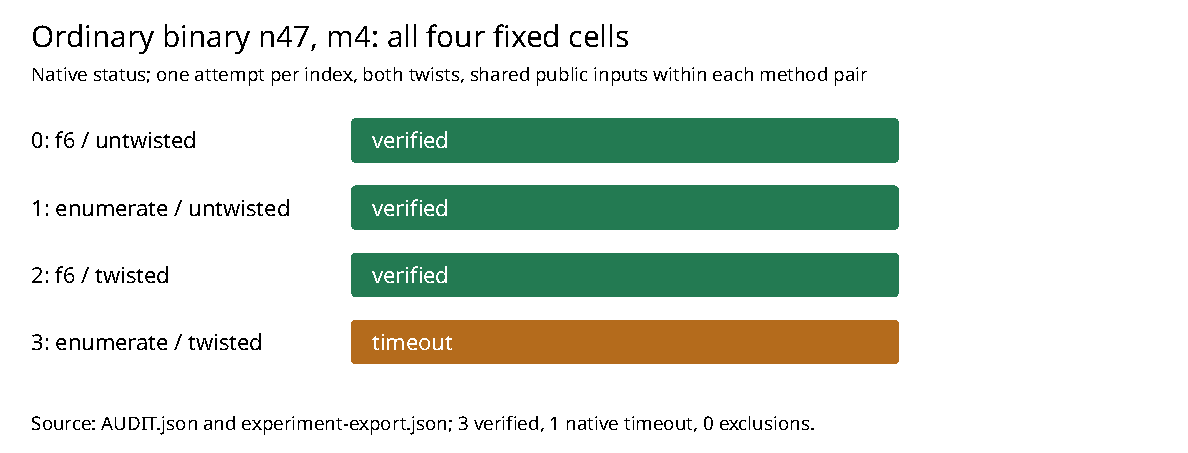
\includegraphics[width=0.95\linewidth]{outcomes.pdf}\end{center}

\subsection*{Evidence and measurement scope}
The independent audit rehashed four archives and 128 native artifacts and
checked paired public inputs, curve/twist identities, point-count certificate
types, and full coefficient-field degree 47. The pinned official export checker
reported zero findings: four planned and attempted, three completed, one
timeout, zero exclusions. Producer S3 receipts cover every archive and pointer;
separate fresh reads sampled indices 0 and 3. Archive bytes total 1,015,585.

Sixteen phase telemetry records retain raw calling-thread readings, but zero
whole-worker instruction labels are eligible for training. The timed-out
enumeration record is censored; F6 private lookup events are not exported.
See \texttt{report/run.md} for hashes, commands, and linked evidence.
\end{document}
